\documentclass[a4paper,11pt]{jsarticle}


% 数式
\usepackage{amsmath,amsfonts,amssymb}
\usepackage{bm}
% 画像
\usepackage[dvipdfmx]{graphicx}
\usepackage[dvipdfmx]{color}
\usepackage{siunitx}
\usepackage{wrapfig}
\usepackage{cases}
\usepackage{dcolumn}
\usepackage{subcaption}
\makeatletter
\newcommand{\figcaption}[1]{\def\@captype{figure}\caption{#1}}
\newcommand{\tblcaption}[1]{\def\@captype{table}\caption{#1}}
\makeatother

% add hyperlinks
\usepackage[dvipdfmx]{hyperref}
\usepackage{pxjahyper}
\hypersetup{
  colorlinks=true,
  linkcolor=blue,
  citecolor=blue,
  breaklinks=true, 
}

\usepackage{listings,jvlisting}
\lstset{
basicstyle={\ttfamily},
identifierstyle={\small},
commentstyle={\smallitshape},
keywordstyle={\small\bfseries},
ndkeywordstyle={\small},
stringstyle={\small\ttfamily},
frame={tb},
breaklines=true,
columns=[l]{fullflexible},
numbers=left,
xrightmargin=0zw,
xleftmargin=3zw,
numberstyle={\scriptsize},
stepnumber=1,
numbersep=1zw,
lineskip=-0.5ex
}

\begin{document}

\title{vGyへの貢献をどう評価するか}
\author{Hiro Hirabayashi}
\date{\today}
\maketitle

\begin{figure}[h]
  \centering
  \begin{tabular}{ccc}
    \begin{minipage}[t]{0.33\textwidth}
      \begin{subcaptionblock}{1\textwidth}
        \centering
        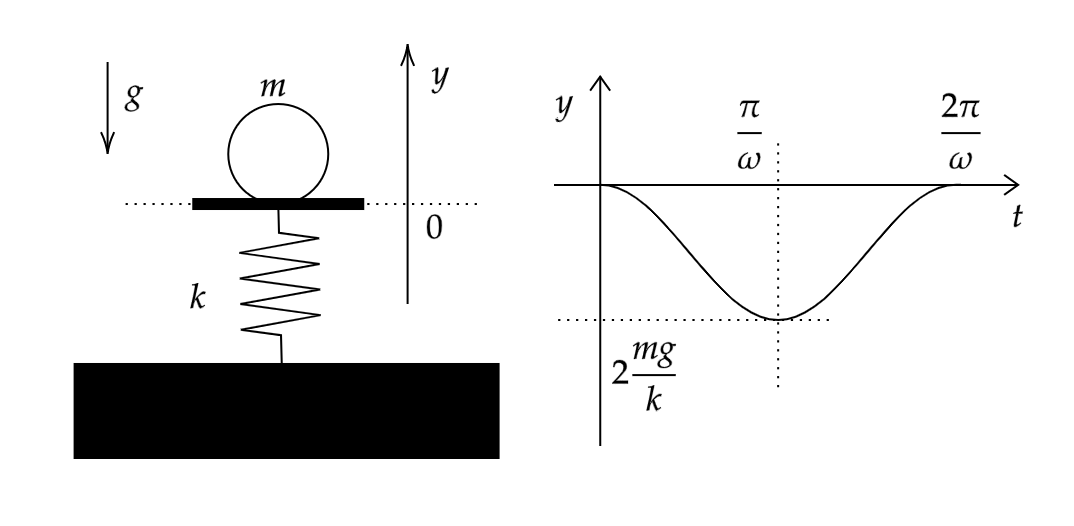
\includegraphics[width=1\textwidth]{simple_string.png}
        \caption{Sec. \ref{section:simple_spring_nonh}}
        \label{simple_string.png}
      \end{subcaptionblock}
    \end{minipage} &
    \begin{minipage}[t]{0.33\textwidth}
      \begin{subcaptionblock}{1\textwidth}
        \centering
        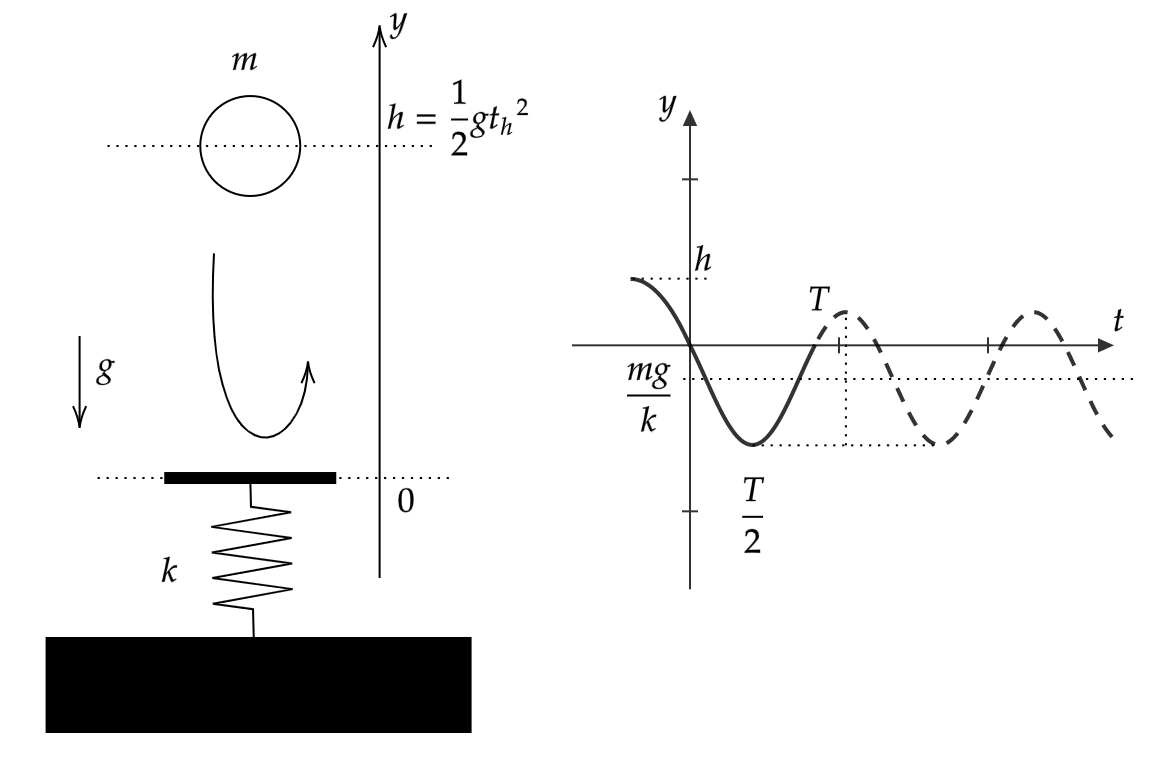
\includegraphics[width=1\textwidth]{fall_and_spring.png}
        \caption{Sec. \ref{section:simple_string_h}}
        \label{fall_and_spring.png}
      \end{subcaptionblock}
    \end{minipage} &
    \begin{minipage}[t]{0.33\textwidth}
      \begin{subcaptionblock}{1\textwidth}
        \centering
        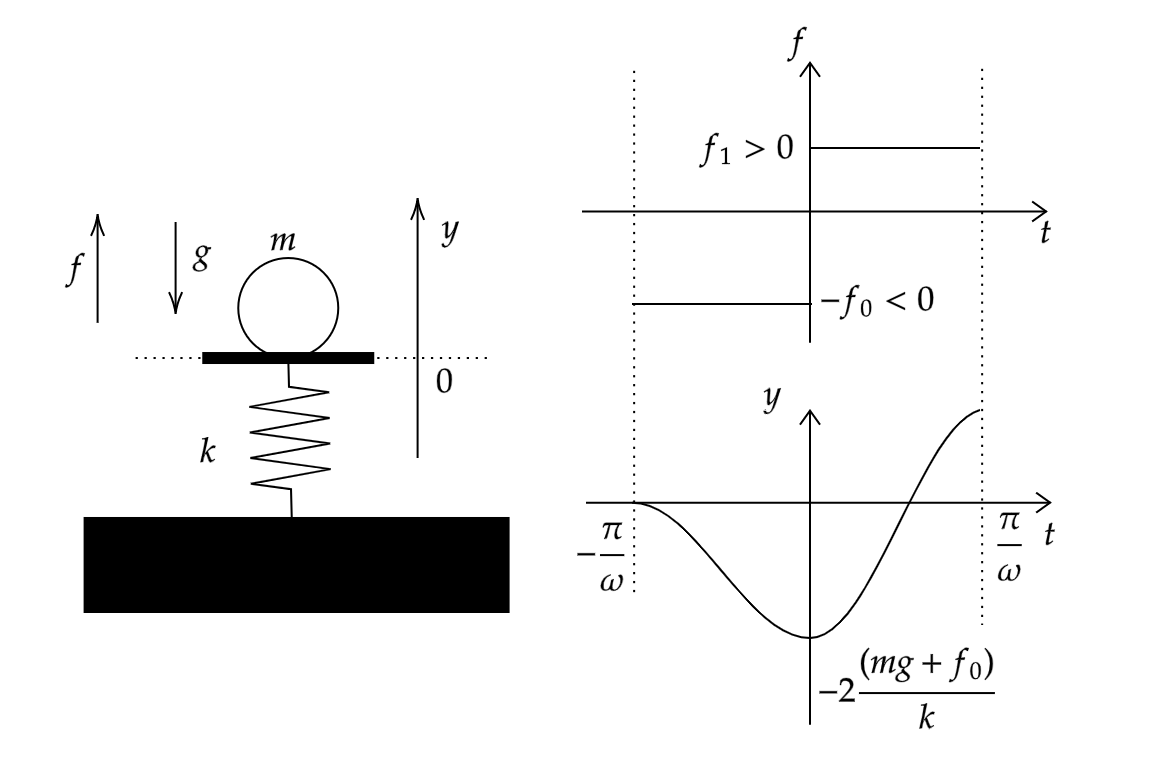
\includegraphics[width=1\textwidth]{spring_given_force.png}
        \caption{Sec. \ref{section:external_forcce}}
        \label{spring_given_force.png}
      \end{subcaptionblock}
    \end{minipage}
  \end{tabular}
  \caption{
    状況説明
  }
\end{figure}

現状考えている評価方法は
\begin{enumerate}
  \item 力積
  \item 仕事量
  \item $\int\sigma (vy_G)ay_G dt$ で表される単位付き力積
\end{enumerate}

\begin{table}[h]
  \centering
  \caption{力積}
  \begin{tabular}{c|c|c|c}
    \hline \hline
    \multicolumn{4}{l}{力積}
    \\ \hline \hline
     & 重力                                             & ばねの弾性 & 外力
    \\ \hline
    Sec. \ref{section:simple_spring_nonh}
     & $-mg \frac{2\pi}{\omega}$
     & $mg \frac{2\pi}{\omega}$
     & -
    \\
    Sec. \ref{section:simple_string_h}
     & $-mg \left(T + t_h\right)$
     & $mgT + 2mgt_h$
     & -
    \\
    Sec. \ref{section:external_forcce}
     & $-mgT - mg\frac{\pi}{\omega}$
     & $mg\frac{\pi}{\omega} + \frac{\pi}{\omega} f_0
      + mgT - f_1 T
      + \frac{2}{\omega} \sqrt{(mg + f_0)(f_1+f_0)}$
     & $-\frac{\pi}{\omega}f_0 + f_1 T$
    \\
    \hline \hline
    \multicolumn{4}{l}{仕事量}
    \\ \hline \hline
     & 重力                                             & ばねの弾性 & 外力
    \\ \hline
    Sec. \ref{section:simple_spring_nonh}
     & $0$
     & $0$
     & -
    \\
    Sec. \ref{section:simple_string_h}
     & $mgh$
     & $0$
     & -
    \\
    Sec. \ref{section:external_forcce}
     & $0$
     & $0$
     & $\frac{2(mg+f_0)}{k}(f_0 + f_1)$
    \\
    \hline \hline
    \multicolumn{4}{l}{単位付き力積}
    \\ \hline \hline
     & 重力                                             & ばねの弾性 & 外力
    \\ \hline
    Sec. \ref{section:simple_spring_nonh}
     & $0$
     & $0$
     & -
    \\
    Sec. \ref{section:simple_string_h}
     & $mgt_h$
     & $0$
     & -
    \\
    Sec. \ref{section:external_forcce}
     & $mg\left( \frac{\pi}{\omega} - T \right)$
     & $mg\frac{\pi}{\omega} + \frac{\pi}{\omega} f_0
      - mgT + f_1 T
      - \frac{2}{\omega} \sqrt{(mg + f_0)(f_1+f_0)}$
     & $f_0 \frac{\pi}{\omega} + f_1 T$
    \\
  \end{tabular}
  \label{}
\end{table}

% \begin{table}[h]
%   \centering
%   \caption{仕事量}
%   \begin{tabular}{c|c|c|c}
%     & 重力 & ばねの弾性 & 外力
%     \\ \hline
%     Sec. \ref{section:simple_spring_nonh}
%     & $0$
%     & $0$
%     &-
%     \\
%     Sec. \ref{section:simple_string_h}
%     & $mgh$
%     & $0$
%     &-
%     \\
%     Sec. \ref{section:external_forcce}
%     & $0$
%     & $0$
%     & $\frac{2(mg+f_0)}{k}(f_0 + f_1)$
%     \\
%   \end{tabular}
%   \label{}
% \end{table}

% \begin{table}[h]
%   \centering
%   \caption{単位付き力積}
%   \begin{tabular}{c|c|c|c}
%     & 重力 & ばねの弾性 & 外力
%     \\ \hline
%     Sec. \ref{section:simple_spring_nonh}
%     & $-mg \frac{2\pi}{\omega}$
%     & $mg \frac{2\pi}{\omega}$
%     &-
%     \\
%     Sec. \ref{section:simple_string_h}
%     & $-mg \left(T + t_h\right)$
%     & $mgT + 2mgt_h$
%     &-
%     \\
%     Sec. \ref{section:external_forcce}
%     & $-mgT - mg\frac{\pi}{\omega}$
%     & $-\frac{\pi}{\omega}f_0 + f_1 T$
%     & $f_0 \frac{\pi}{\omega} + f_1 T$
%     \\
%   \end{tabular}
%   \label{}
% \end{table}

\clearpage
\section{Case: 単純なばね(落下なし)}
\label{section:simple_spring_nonh}

\begin{figure}[h]
  \centering
  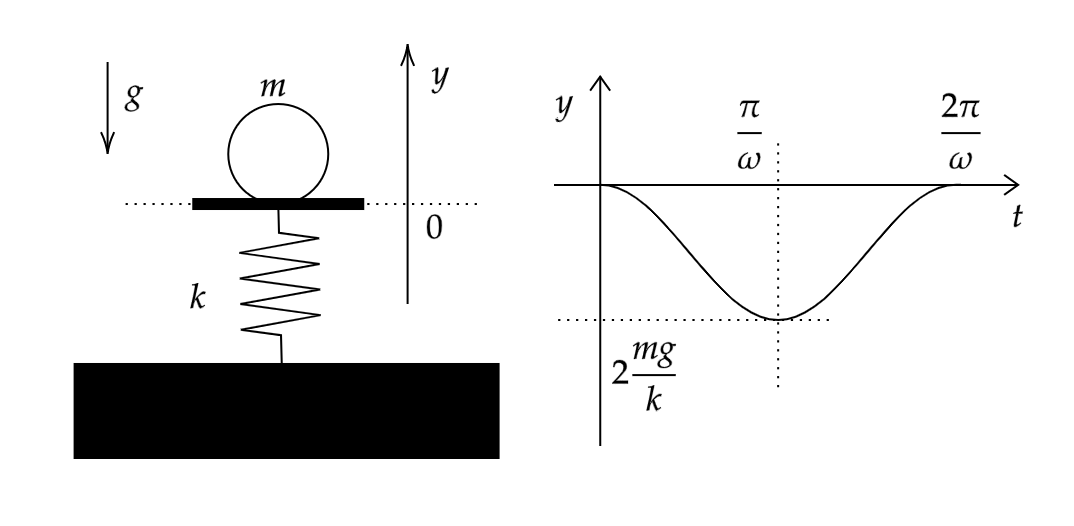
\includegraphics[width = 0.6\textwidth]{simple_string.png}
  \caption{}
  \label{simple_string.png}
\end{figure}

\subsection{準備}
\begin{align}
  ma & = -mg - ky
  \\ &= -k\left(y + \frac{mg}{k}\right)
\end{align}
\begin{align}
  \therefore
  \left(y+\frac{mg}{k}\right) = A\sin(\omega t) + B\cos(\omega t)
\end{align}
ただし、$t=0$で$y=0,\dot{y}=0$より、
\begin{align}
  y & = -\frac{mg}{k} + \frac{mg}{k}\cos(\omega t)
  \\ &= \frac{mg}{k}\left(-1+\cos(\omega t)\right)
\end{align}

そんで、ばね板から離れる条件はもちろん
\begin{align}
  F_y = 0 \Leftrightarrow ky = 0
\end{align}
*ばね板にちゃんと質量(M)を持たせると、
\begin{align}
  \begin{cases}
    M\ddot{y} & = -F_y - ky
    \\ m\ddot{y} &= F_y
  \end{cases}
\end{align}
\begin{align}
  \therefore (M + m)\ddot{y} = - ky
\end{align}
になって質量が変わるだけ。だけどシミュレーションするときには板に質量をもたせておいたほうが安心かな。

離ばねまでちょうど1周期だから
$\frac{2\pi}{\omega}$
だけかかる。

\subsection{貢献}
先に結論だけ書く。
力積だと重力がいたずらに負に評価されて、
仕事量、単位付き力積だとどっちも0になる。
仕事量、単位付き力積がうまく評価できている。

\subsubsection{力積}
重力による力積は
\begin{align}
  \int_0^{\frac{2\pi}{\omega}} -mg dt = -mg \frac{2\pi}{\omega}
\end{align}

ばねの弾性による力積は
\begin{align}
  \int_0^{\frac{2\pi}{\omega}} -ky dt & = -k \int_0^{\frac{2\pi}{\omega}} \frac{mg}{k}\left(-1+\cos(\omega t)\right)
  \\ &= -mg \int_0^{\frac{2\pi}{\omega}} \left(-1+\cos(\omega t)\right) dt
  \\ &= -mg \left[-t+\frac{1}{\omega}\sin(\omega t)\right]_0^{\frac{2\pi}{\omega}}
  \\ &= -mg \left( -\frac{2\pi}{\omega} \right) = mg \frac{2\pi}{\omega}
\end{align}

離ばね地点において元の状態に戻っているから、正味の力積が0になるのは妥当。

\subsubsection{仕事量}
重力による仕事量は
\begin{align}
  \int_0^{\frac{2\pi}{\omega}} -mg\cdot\dot{y} dt = \int_{t=0}^{t=\frac{2\pi}{\omega}} -mg dy = 0
\end{align}
位置エネルギーの変化分だから0になるのは妥当。

ばねの弾性による仕事量も
\begin{align}
  \int_0^{\frac{2\pi}{\omega}} -ky \cdot\dot{y} dt
   & = \int_{t=0}^{t=\frac{2\pi}{\omega}} -kydy
  \\&= \left[-\frac{1}{2}ky^2\right]_{t=0}^{t=\frac{2\pi}{\omega}} = 0
\end{align}
位置エネルギーの変化分だから0になるのは妥当。

離ばね地点において元の状態に戻っているから、正味の仕事量が0になるのは妥当。

\subsubsection{$\int\sigma (vy_G)ay_G dt$ で表される単位付き力積}
重力による単位付き力積は
\begin{align}
  \int_0^{\frac{\pi}{\omega}} -mg\cdot(-1) dt + \int_{\frac{\pi}{\omega}}^{\frac{2\pi}{\omega}} -mg\cdot(1) dt
   & = mg\frac{\pi}{\omega} + \left(-mg\frac{\pi}{\omega}\right) = 0
\end{align}

ばねの弾性による単位付き力積は
\begin{align}
  \int_0^{\frac{\pi}{\omega}} -ky\cdot(-1) dt
   & + \int_{\frac{\pi}{\omega}}^{\frac{2\pi}{\omega}} -ky\cdot(1) dt
  \\ &= k \int_0^{\frac{\pi}{\omega}} \frac{mg}{k}\left(-1+\cos(\omega t)\right)
  - k \int_{\frac{\pi}{\omega}}^{\frac{2\pi}{\omega}} \frac{mg}{k}\left(-1+\cos(\omega t)\right)
  \\&= mg \left[-t+\frac{1}{\omega}\sin(\omega t)\right]_0^{\frac{\pi}{\omega}}
  - mg \left[-t+\frac{1}{\omega}\sin(\omega t)\right]_{\frac{\pi}{\omega}}^{\frac{2\pi}{\omega}}
  \\&= mg \left( -\frac{\pi}{\omega} + 0 \right)
  - mg\left( -\frac{\pi}{\omega} + 0 \right)
  \\ &= 0
\end{align}


\section{Case: 単純なばね(落下あり)}
\label{section:simple_string_h}

\begin{figure}[h]
  \centering
  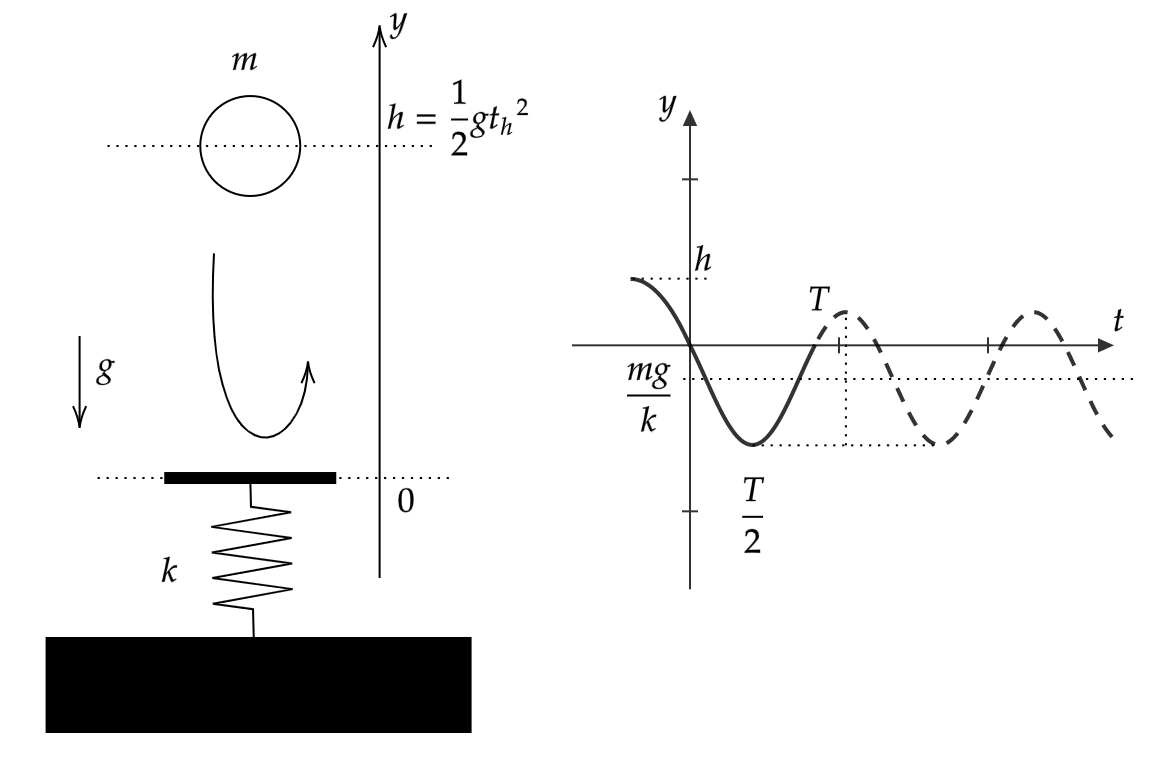
\includegraphics[width = 0.6\textwidth]{fall_and_spring.png}
  \caption{}
  \label{fall_and_spring.png}
\end{figure}

\subsection{準備}
\subsubsection{落下時}

\begin{align}
  y
   & = h - \frac{1}{2}gt^2
  \\ &= \frac{1}{2}g{t_h}^2 - \frac{1}{2}gt^2
\end{align}
つまり落下区間は$0\leq t \leq t_h$となるが、
あとあと面倒なので、落下区間を$-t_h\leq t \leq 0$とする。
$t = 0$の時
$vy = -gt_h$

\subsubsection{ばね板についてるとき}
\begin{align}
  ma & = -mg - ky
  \\ &= -k\left(y + \frac{mg}{k}\right)
\end{align}
\begin{align}
  \therefore
  \left(y+\frac{mg}{k}\right) = A\sin(\omega t) + B\cos(\omega t)
\end{align}
ただし、$t=0$で$y=0,\dot{y}=-gt_h$より、
\begin{align}
  y & = -\frac{mg}{k} - \frac{gt_h}{\omega}\sin(\omega t) + \frac{mg}{k}\cos(\omega t)
  \\ &= -\frac{mg}{k} + \sqrt{\left(\frac{gt_h}{\omega}\right)^2 + \left(\frac{mg}{k}\right)^2}\cos \left( \omega t + A \right)
\end{align}

\begin{align}
  \cos\left( \omega t + A \right)
   & = \cos \omega t \cos A - \sin \omega t \sin A
  \\&= \frac{\frac{mg}{k}}{\sqrt{\left(\frac{gt_h}{\omega}\right)^2 + \left(\frac{mg}{k}\right)^2}}\cos\omega t
  - \frac{\frac{gt_h}{\omega}}{\sqrt{\left(\frac{gt_h}{\omega}\right)^2 + \left(\frac{mg}{k}\right)^2}}\sin \omega t
\end{align}
\begin{align}
  \cos A & = \frac{\frac{mg}{k}}{\sqrt{\left(\frac{gt_h}{\omega}\right)^2 + \left(\frac{mg}{k}\right)^2}}
  \\ \sin A &= \frac{\frac{gt_h}{\omega}}{\sqrt{\left(\frac{gt_h}{\omega}\right)^2 + \left(\frac{mg}{k}\right)^2}}
\end{align}

そんで、ばね板から離れる条件はもちろん
\begin{align}
  F_y = 0 \Leftrightarrow ky = 0 \Leftrightarrow y = 0
\end{align}

*ばね板にちゃんと質量(M)を持たせると、
衝突は完全非弾性衝突かつ運動量の保存を考える必要がある。

着ばねから離ばねまでの時間はきれいにあらわされないが、$T$でおくと、
\begin{align}
   & \begin{cases}
        & -\frac{mg}{k} + \sqrt{\left(\frac{gt_h}{\omega}\right)^2 + \left(\frac{mg}{k}\right)^2} \cos \left( \omega T + A \right) = 0
       \\& 0 + \omega \sqrt{\left(\frac{gt_h}{\omega}\right)^2 + \left(\frac{mg}{k}\right)^2} \left( - \sin \left( \omega T + A \right) \right) = gt_h
     \end{cases}
  \\& \Leftrightarrow
  \begin{cases}
    \cos \left( \omega T + A \right) & = \frac{ \frac{mg}{k} }{ \sqrt{\left(\frac{gt_h}{\omega}\right)^2 + \left(\frac{mg}{k}\right)^2} }
    \\ \sin \left( \omega T + A \right) &= - \frac{gt_h}{ \omega \sqrt{\left(\frac{gt_h}{\omega}\right)^2 + \left(\frac{mg}{k}\right)^2} }
  \end{cases}
\end{align}

また、最下点に至る時刻は$t=\frac{T}{2}$で、その時に
$y=-\frac{mg}{k} + \sqrt{\left(\frac{gt_h}{\omega}\right)^2 + \left(\frac{mg}{k}\right)^2}$
かつ
$\dot{y} = 0$
より、
\begin{align}
  \cos \left( \omega \frac{T}{2} + A \right) & = 1
  \\
  \sin \left( \omega \frac{T}{2} + A \right) & = 0
\end{align}

\subsection{貢献}
先に結論だけ書く。
力積だと重力がいたずらに負に評価されて、
仕事量、単位付き力積だと重力がいい感じに正に評価される。
仕事量、単位付き力積がうまく評価できている。
\subsubsection{力積}
重力による力積は
\begin{align}
  \int_{-t_h}^{T} -mg dt = -mg \left(T + t_h\right)
\end{align}

ばねの弾性による力積は
\begin{align}
   & \int_0^T -ky dt
  \\ & = -k \int_0^T
  \left( -\frac{mg}{k} + \sqrt{\left(\frac{gt_h}{\omega}\right)^2 + \left(\frac{mg}{k}\right)^2} \cos \left( \omega t + A \right) \right) dt
  \\ & = mgT - k \sqrt{\left(\frac{gt_h}{\omega}\right)^2 + \left(\frac{mg}{k}\right)^2} \int_0^T \cos \left( \omega t + A \right) dt
  \\ & = mgT - k \sqrt{\left(\frac{gt_h}{\omega}\right)^2 + \left(\frac{mg}{k}\right)^2} \left[ \frac{1}{\omega} \sin (\omega t + A) \right]_0^T
  \\ & \begin{aligned}
    = mgT -
     & \left\{ \frac{k}{\omega} \sqrt{\left(\frac{gt_h}{\omega}\right)^2 + \left(\frac{mg}{k}\right)^2}
    \cdot \left[- \frac{gt_h}{ \omega \sqrt{\left(\frac{gt_h}{\omega}\right)^2 + \left(\frac{mg}{k}\right)^2} } \right] \right.
    \\
     & \ \left. - \frac{k}{\omega} \sqrt{\left(\frac{gt_h}{\omega}\right)^2 + \left(\frac{mg}{k}\right)^2}
    \cdot \left[ \frac{\frac{gt_h}{\omega}}{\sqrt{\left(\frac{gt_h}{\omega}\right)^2 + \left(\frac{mg}{k}\right)^2}} \right] \right\}
  \end{aligned}
  \\& = mgT - \left\{ - \frac{2k}{\omega^2} gt_h \right\}
  \\& = mgT + 2mgt_h
\end{align}

合計が
\begin{align}
  \int_{-t_h}^{T} -mg dt + \int_0^T -ky dt
  = \left( -mgT - mgt_h \right) + \left( mgT + 2mgt_h \right) = mgt_h
\end{align}
でちゃんと跳ね返った後の運動量に一致するからオッケー

\subsubsection{仕事量}
重力による仕事量は
\begin{align}
  \int_{-t_h}^{T} -mg \cdot \dot{y} dt
   & = \int_{t=-t_h}^{t=T} -mgdy
  \\
   & = -mg(0 - h) = mgh
\end{align}

ばねの弾性による仕事量は
\begin{align}
  \int_{0}^{T} -ky \cdot \dot{y} dt
   & = \int_{t=0}^{t=T} -kydy
  \\
   & = \left[ -\frac{1}{2} ky^2 \right]_{t=0}^{t=T}
  = -\frac{1}{2}k (0 - 0) = 0
\end{align}

\subsubsection{$\int\sigma (vy_G)ay_G dt$ で表される単位付き力積}
重力による単位付き力積は
\begin{align}
  \int_{-t_h}^{T/2} -mg \cdot (-1) dt
  + \int_{T/2}^{T} -mg \cdot (1) dt
   & = mg\left[ \frac{T}{2} - (-t_h) \right] - mg \left[ T - \frac{T}{2} \right]
  \\
   & = mg\frac{T}{2} + mgt_h - mg\frac{T}{2} = mgt_h
\end{align}

ばねの弾性による単位付き力積は
\begin{align}
   & \int_{0}^{T/2} -ky \cdot (-1) dt
  + \int_{T/2}^{T} -ky \cdot (1) dt
  \\
   & = -k \left\{
  \int_{0}^{T/2} -y dt + \int_{T/2}^{T} y dt
  \right\}
  \\
   &
  \begin{aligned}
    = -k \Bigg\{
     & - \int_{0}^{T/2} \left(
    -\frac{mg}{k} + \sqrt{\left(\frac{gt_h}{\omega}\right)^2 + \left(\frac{mg}{k}\right)^2}\cos \left( \omega t + A \right)
    \right) dt
    \\
     & + \int_{T/2}^{T} \left(
    -\frac{mg}{k} + \sqrt{\left(\frac{gt_h}{\omega}\right)^2 + \left(\frac{mg}{k}\right)^2}\cos \left( \omega t + A \right)
    \right) dt \Bigg\}
  \end{aligned}
  \\
   & \begin{aligned}
       = -k \Bigg\{
        & - \left[
         -\frac{mg}{k}t + \frac{1}{\omega} \sqrt{\left(\frac{gt_h}{\omega}\right)^2 + \left(\frac{mg}{k}\right)^2} \sin (\omega t + A)
         \right]_0^{T/2}
       \\
        & + \left[
         -\frac{mg}{k}t + \frac{1}{\omega} \sqrt{\left(\frac{gt_h}{\omega}\right)^2 + \left(\frac{mg}{k}\right)^2} \sin (\omega t + A)
         \right]_{T/2}^T
       \Bigg\}
     \end{aligned}
  \\
   & \begin{aligned}
       = -k \Bigg\{
        & - \left[
         -\frac{mg}{k}\frac{T}{2} + \frac{1}{\omega} \sqrt{\left(\frac{gt_h}{\omega}\right)^2 + \left(\frac{mg}{k}\right)^2} (\sin(\frac{\omega T}{2} + A) - \sin(A))
         \right]
       \\
        & + \left[
         -\frac{mg}{k}\frac{T}{2} + \frac{1}{\omega} \sqrt{\left(\frac{gt_h}{\omega}\right)^2 + \left(\frac{mg}{k}\right)^2} (\sin(\omega T + A) - \sin(\frac{\omega T}{2} + A))
         \right]
       \Bigg\}
     \end{aligned}
  \\
   & \left( \because \cos (\frac{\omega T}{2} + A) = -1, \ \sin (\frac{\omega T}{2} + A) = 0 \right)
  \\
   & = -k \frac{1}{\omega} \sqrt{\left(\frac{gt_h}{\omega}\right)^2 + \left(\frac{mg}{k}\right)^2} \left(\sin A + \sin (\omega T + A)\right)
  \\
   & \left(
  \begin{aligned}
      \because \sin A + \sin (\omega T + A) =
       & \frac{\frac{gt_h}{\omega}}{\sqrt{\left(\frac{gt_h}{\omega}\right)^2 + \left(\frac{mg}{k}\right)^2}}
      \\
       & + \left( - \frac{gt_h}{ \omega \sqrt{\left(\frac{gt_h}{\omega}\right)^2 + \left(\frac{mg}{k}\right)^2} } \right)
      = 0
    \end{aligned}
  \right)
  \\
   & = 0
\end{align}

\section{Case: 外力が与えられたとき}
\label{section:external_forcce}

\begin{figure}[h]
  \centering
  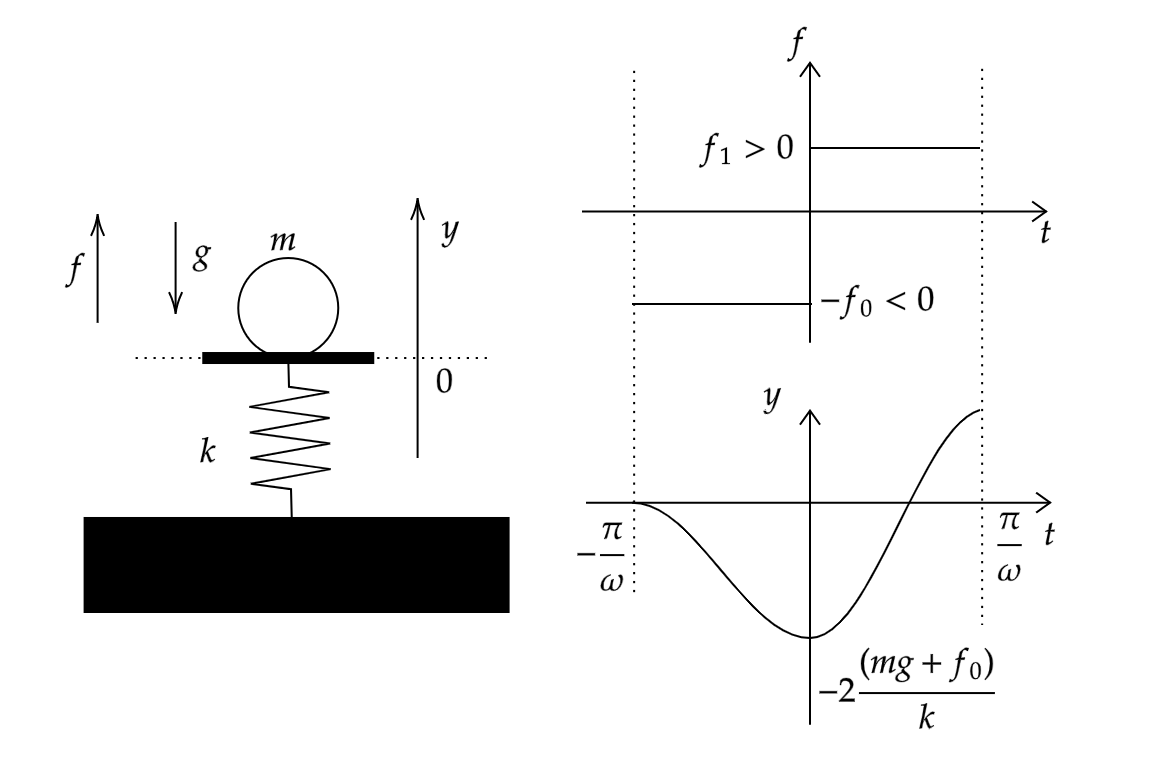
\includegraphics[width = 0.6\textwidth]{spring_given_force.png}
  \caption{}
  \label{spring_given_force.png}
\end{figure}
\subsection{準備}
\subsubsection{$-\frac{\pi}{\omega} < t < 0$}
\begin{align}
  m\ddot{y}
   & = - mg - ky - f_0
  \\
   & = -k\left( y + \frac{mg+f_0}{k} \right)
\end{align}
\begin{align}
  y = - \frac{mg+f_0}{k} + A \sin \omega t + B \cos \omega t
\end{align}
$t=0$で$y=-2\frac{mg+f_0}{k}, \dot{y} = 0$より
\begin{align}
  y
   & = - \frac{mg+f_0}{k} - \frac{mg+f_0}{k} \cos \omega t
  \\
   & = -\frac{mg+f_0}{k} \left( 1 + \cos \omega t \right)
\end{align}

\subsubsection{$0 < t$}
\begin{align}
  m\ddot{y}
   & = - mg - ky + f_1
  \\
   & = -k\left( y + \frac{mg - f_1}{k} \right)
\end{align}
\begin{align}
  y = - \frac{mg - f_1}{k} + A \sin \omega t + B \cos \omega t
\end{align}
$t=0$で$y=-2\frac{mg + f_0}{k}, \dot{y} = 0$より
\begin{align}
   & -2\frac{mg + f_0}{k} = -\frac{mg - f_1}{k} + B
  \\
   & \Rightarrow
  B = -\frac{mg + 2f_0 + f_1}{k}
\end{align}
\begin{align}
  \therefore y
   & = - \frac{mg - f_1}{k} - \frac{mg + 2f_0 + f_1}{k} \cos \omega t
\end{align}

離ばねの定義は今までと同様に
\begin{align}
  ky=0 \Rightarrow y=0
\end{align}
だから、時刻$t=T$で離ばねする場合
\begin{align}
  0 & = -\frac{mg - f_1}{k} - \frac{mg + 2f_0 + f_1}{k} \cos \omega T
  \\
  \Leftrightarrow
  \cos \omega T
    & = -\frac{mg - f_1}{mg + 2f_0 + f_1}
\end{align}
また、$T<\frac{\pi}{\omega}$より$\sin \omega T > 0$だから
\begin{align}
  \sin \omega T
   & = \sqrt{1 - \cos^2 \omega T}
  \\
   & = \sqrt{ \frac{(mg + 2f_0 + f_1)^2 - (mg - f_1)^2}{(mg + 2f_0 + f_1)^2}}
  \\
   & = \sqrt{
  \frac{m^2g^2 + 4mgf_0 + 2mgf_1 + 4f_0f_1 + 4{f_0}^2 + {f_1}^2 - m^2g^2 + 2mgf_1 - {f_1}^2}
  {(mg + 2f_0 + f_1)^2}
  }
  \\
   & = \sqrt{
    \frac{4mgf_0 + 4mgf_1 + 4f_0f_1 + 4{f_0}^2}{(mg + 2f_0 + f_1)^2}
  }
  \\
   & = \frac{2\sqrt{mgf_0 + mgf_1 + f_0f_1 + {f_0}^2}}{mg + 2f_0 + f_1}
  \\
   & = \frac{2\sqrt{(mg + f_0)(f_1+f_0)}}{mg + 2f_0 + f_1}
\end{align}

また、離ばね時の運動量は離ばね時の速度$v_f$を用いてエネルギー保存則より
\begin{align}
  \frac{1}{2}m{v_f}^2
   & = mg\left(-2\frac{mg+f_0}{k}\right)
  + f_1\cdot 2\frac{mg+f_0}{k} + \frac{1}{2}k\left( \frac{4(mg+f_0)^2}{k^2} \right)
  \\
   & = \frac{mg+f_0}{k}\left( -2mg + 2f_1 + 2mg + 2f_0 \right)
  \\
   & = \frac{mg+f_0}{k}\left( 2f_1 + 2f_0 \right)
  \\
  v_f
   & = 2\sqrt{\frac{(mg + f_0) (f_1 + f_0)}{mk}}
  \\
   & = \frac{2}{\omega}\omega \sqrt{\frac{(mg + f_0) (f_1 + f_0)}{mk}}
  \\
   & = \frac{2}{\omega} \sqrt{\frac{k}{m}} \sqrt{\frac{(mg + f_0) (f_1 + f_0)}{mk}}
  \\
   & = \frac{2}{m\omega}\sqrt{(mg + f_0)(f_1 + f_0)}
  \\ \therefore
  mv_f
   & = \frac{2}{\omega} \sqrt{(mg + f_0)(f_1 + f_0)}
\end{align}

\subsection{貢献}

\subsubsection{力積}
合計が
\begin{align}
  mv_f
   & = \frac{2}{\omega} \sqrt{(mg + f_0)(f_1 + f_0)}
\end{align}
に等しくなるはず。

重力による力積は
\begin{align}
  \int_{-\frac{\pi}{\omega}}^{T} -mgdt = -mgT - mg\frac{\pi}{\omega}
\end{align}

外力による力積は
\begin{align}
  \int_{-\frac{\pi}{\omega}}^{0} -f_0 dt
  + \int_0^T f_1 dt
   & = -\frac{\pi}{\omega}f_0 + f_1 T
\end{align}

ばねの弾性による力積は
\begin{align}
   & \int_{-\frac{\pi}{\omega}}^0 -ky dt
  + \int_0^T -ky dt
  \\
   & = \int_{-\frac{\pi}{\omega}}^0 (mg + f_0)( 1 + \cos \omega t ) dt
  + \int_0^T \Big\{ (mg-f_1) + (mg + 2f_0 + f_1)\cos \omega t\Big\} dt
  \\
   & = (mg + f_0)\left[ t + \frac{1}{\omega} \sin \omega t\right]_{\frac{\pi}{\omega}}^0
  + (mg - f_1)\left[ t \right]_0^T
  + (mg + 2f_0 + f_1) \frac{1}{\omega} \left[ \sin \omega t \right]_0^T
  \\
   & = mg\frac{\pi}{\omega} + \frac{\pi}{\omega} f_0
  + mgT - f_1 T
  + \frac{mg + 2f_0 + f_1}{\omega} \sin \omega T
  \\
   & = mg\frac{\pi}{\omega} + \frac{\pi}{\omega} f_0
  + mgT - f_1 T
  + \frac{mg + 2f_0 + f_1}{\omega} \frac{2\sqrt{(mg + f_0)(f_1+f_0)}}{mg + 2f_0 + f_1}
  \\
   & = mg\frac{\pi}{\omega} + \frac{\pi}{\omega} f_0
  + mgT - f_1 T
  + \frac{2}{\omega} \sqrt{(mg + f_0)(f_1+f_0)}
\end{align}

合計もちゃんと一致した。

\subsubsection{仕事量}
重力による仕事量は
\begin{align}
  \int_{-\frac{\pi}{\omega}}^{T} -mg\cdot \dot{y} dt
   & = \int_{t=-\frac{\pi}{\omega}}^{t=T} -mgdy
  \\
   & =-mg\left[ y \right]_{t=-\frac{\pi}{\omega}}^{t=T}
  \\
   & = -mg\left[ 0 - 0 \right] = 0
\end{align}

外力による仕事量は
\begin{align}
   & \int_{-\frac{\pi}{\omega}}^{0} -f_0 \cdot \dot{y} dt
  + \int_{0}^{T} f_1 \cdot \dot{y} dt
  \\
   & = \int_{t=-\frac{\pi}{\omega}}^{t=0} -f_0 dy
  + \int_{t=0}^{t=T} f_1 dy
  \\
   & = -f_0 \left[ y \right]_{t=-\frac{\pi}{\omega}}^{t=0}
  + f_1 \left[ y \right]_{t=0}^{t=T}
  \\
   & = -f_0 \left[ -\frac{2(mg + f_0)}{k} - 0 \right]
  + f_1 \left[ 0 - \left( -\frac{2(mg + f_0)}{k} \right) \right]
  \\
   & =\frac{2(mg + f_0)}{k}(f_0 + f_1)
  \\
   & \Bigl( = \frac{1}{2}m{v_f}^2 \Bigr)
\end{align}

ばねの弾性による仕事量は
\begin{align}
  \int_{-\frac{\pi}{\omega}}^{T} -ky \cdot \dot{y} dt
   & = \int_{t=-\frac{\pi}{\omega}}^{t=T} -ky dy
  \\
   & = -\frac{1}{2}k \left[ y^2 \right]_{t=-\frac{\pi}{\omega}}^{t=T}
  \\
   & = -\frac{1}{2}k \left[ 0 - 0 \right] = 0
\end{align}

\subsubsection{$\int\sigma (vy_G)ay_G dt$ で表される単位付き力積}
重力による単位付き力積は
\begin{align}
   & \int_{-\frac{\pi}{\omega}}^{0} -mg \cdot (-1) dt
  + \int_{0}^{T} -mg \cdot (1) dt
  \\
   & = mg\frac{\pi}{\omega} - mgT = mg\left( \frac{\pi}{\omega} - T\right)
\end{align}

ばねの弾性による単位付き力積は
\begin{align}
   & \int_{-\frac{\pi}{\omega}}^0 -ky \cdot (-1) dt
  + \int_0^T -ky \cdot (1) dt
  \\
   & = \int_{-\frac{\pi}{\omega}}^0 (mg + f_0)( 1 + \cos \omega t ) dt
  - \int_0^T \Big\{ (mg-f_1) + (mg + 2f_0 + f_1)\cos \omega t\Big\} dt
  \\
   & = (mg + f_0)\left[ t + \frac{1}{\omega} \sin \omega t\right]_{\frac{\pi}{\omega}}^0
  - (mg - f_1)\left[ t \right]_0^T
  - (mg + 2f_0 + f_1) \frac{1}{\omega} \left[ \sin \omega t \right]_0^T
  \\
   & = mg\frac{\pi}{\omega} + \frac{\pi}{\omega} f_0
  - mgT + f_1 T
  - \frac{mg + 2f_0 + f_1}{\omega} \sin \omega T
  \\
   & = mg\frac{\pi}{\omega} + \frac{\pi}{\omega} f_0
  - mgT + f_1 T
  - \frac{mg + 2f_0 + f_1}{\omega} \frac{2\sqrt{(mg + f_0)(f_1+f_0)}}{mg + 2f_0 + f_1}
  \\
   & = mg\frac{\pi}{\omega} + \frac{\pi}{\omega} f_0
  - mgT + f_1 T
  - \frac{2}{\omega} \sqrt{(mg + f_0)(f_1+f_0)}
\end{align}

外力による単位付き力積は
\begin{align}
   & \int_{-\frac{\pi}{\omega}}^{0} -f_0 \cdot (-1) dt
  + \int_{0}^{T} f_1 \cdot (1) dt
  \\
   & = f_0 \left[ t \right]_{-\frac{\pi}{\omega}}^{0}
  + f_1 \left[ t \right]_{0}^{T}
  \\
   & = f_0 \frac{\pi}{\omega} + f_1 T
\end{align}

\end{document}F